\section{Scaling under explicit resource constraints}
\label{sec:scaling}
\subsection{Quality, latency, and cost are separate outcomes}
The practical choice is a policy on a resource--quality frontier. For a configuration $x$, write its measured outcome as $Q_x(B,T)$, where $B$ is a specified budget and $T$ a deadline. A comparison at fixed $T$ asks what the system can deliver before a deadline, permitting different spending. A comparison at fixed $B$ asks how effectively it uses that resource. Time to reach a quality threshold asks a third question. These views should be reported together when possible; none can be substituted for another.

Table~\ref{tab:scaling} preserves the principal contrasts. OpenAI's published GPT-5.6 Sol curves compare one, four, and, on two of three tasks, sixteen agents across effort levels; read along the curves at equal total output tokens, the single-agent curve is higher \citep{openai-gpt56-ultra,ord-swarm-scaling}. This is a reading of published curves, not a run at a matched budget. The latency and dollar axes in that release are simulated from operational data rather than timed in a randomized study.

Avalon-M1, from General Reasoning, Inc., adds a direct matched-token control for a trained organization \citep{avalon-m1}. Its Avalon-M1-Mini model (120B parameters, 12B active) works either alone or as a CEO agent that may hire up to eight specialists from the same policy. In the control, a single agent may not submit until it has produced as many output tokens as the eight-hire organization. The organization scores higher on FrontierScience (63.5\% versus 55.5\%; 160 tasks, one run each), lower on the hard subset of SWE-Bench Pro V2 (23.5\% versus 37.3\%; 51 tasks, one run each), and about the same on IMO-ProofBench-Advanced, where proofs are graded on a 0--7 scale (37.5\% versus 37.7\% of the maximum; 30 problems, four runs each). No intervals are reported, but the direction of the team effect at equal output tokens differs across tasks. Against ordinary single-agent execution without the extra tokens, the same organization is better on 14 of 16 percentage-scored benchmarks, by 3.9 points on average. The report describes a model that is still in training.

The Opus 5.5 ProgramBench comparison makes the tradeoff visible at a fixed threshold: five peers reach 60\% of hidden tests 2.7 times faster than one agent while using about 1.9 times as many tokens. The developer reports the speed ratio; the token ratio is read from its plot. The trajectories approach a similar final score \citep{opus55-card}. On the same developer's knowledge-building and Lean tasks, growing the team from one to ten agents substantially improves the result within 24 hours, and further growth yields smaller gains; token costs for the larger groups are not disclosed.

\begin{table*}[t]
\centering\small
\begin{tabularx}{\textwidth}{@{}p{0.2\textwidth}p{0.25\textwidth}Y@{}}
\toprule
Evidence unit & Resource condition & Outcome and inference boundary\\
\midrule
GPT-5.6 Sol \citep{openai-gpt56-ultra} & Total output tokens; 1/4/16 agents, with 16 absent on one task & One agent is more token-efficient on the reported curves; simulated latency can favor parallel execution.\\\addlinespace[2pt]
Avalon-M1 \citep{avalon-m1} & Equal output tokens: organization with up to eight hires versus one agent forced to spend as much & FrontierScience 63.5\% versus 55.5\% (160 tasks); SWE-Bench Pro V2 hard subset 23.5\% versus 37.3\% (51 tasks); IMO-ProofBench 37.5\% versus 37.7\% of the maximum grade (30 problems $\times$ 4 runs). Direction depends on the task.\\\addlinespace[2pt]
Opus 5.5, ProgramBench \citep{opus55-card} & Time and tokens to the same 60\% hidden-test score & Five peers versus one agent: $2.7\times$ faster at about $1.9\times$ tokens (token ratio read from plot); common eventual score.\\\addlinespace[2pt]
Opus 5, BrowseComp \citep{opus5-card-multiagent} & Equal nominal 10M-token cap; actual spending differs & Ten agents: 93.6\% versus 90.5\%; roughly $2.5\times$ cost from the source plot. An improved observed outcome, not equal-cost superiority.\\\addlinespace[2pt]
Parallel agent teams \citep{parallel-agent-teams} & Budget of 100 Qwen3.8-27B agents; a verifier keeps the best solution & Best of ten teams of ten beats best of 100 single agents on 10 of 12 tasks and one team of 100 on all four tasks where it ran. Best-of results, not averages.\\\addlinespace[2pt]
Coding teams, Cohere \citep{coding-team-compute-allocation} & Measured cost on ProgramBench & Teams beat solo agents at three to seven times the cost; delegating only planning matches full delegation at about half its cost.\\\addlinespace[2pt]
Kim et al. \citep{kim-scaling-agent-systems} & Shared token limit, matched tasks and tools & Mean relative gain 0.0\% across diverse settings; effects from $-70.0\%$ to $+80.8\%$. Heterogeneity dominates the average.\\\addlinespace[2pt]
Agents serving users \citep{collaboration-serving-users} & Same model on $\tau^2$-bench with a fixed simulated user & A centralized multi-agent system is worse in 12 of 13 mechanically valid cells; the thirteenth is $+2.7$ points (95\% CI $-6.7$ to $+12.7$). No cell met the fidelity bar for executing the planner's orders.\\\addlinespace[2pt]
Park et al., ARC-AGI-3 \citep{test-time-communication} & Same number of agents; output-token curves also reported & Five communicating agents: 8.0\% solved versus 2.2\% for best@5; crossover depends on budget and task.\\\addlinespace[2pt]
ScaleMAS \citep{scalemas-substrate} & About 20M tokens per example, BrowseComp-Plus & Eight ScaleMAS agents reach 60.0\% versus 26.0\% for sixteen DeLM agents.\\\addlinespace[2pt]
SAT \citep{sat-teams} & Approximately matched sequential role execution & 66.7\% versus 58.7\% averaged over math and physics; the advantage shrinks or disappears on some individual sets.\\\addlinespace[2pt]
DeLM \citep{delm-shared-context} & Measured price, SWE-bench Verified & Two peers: 63.72\% versus 55.26\% for the orchestration baseline at \$0.24 per task; distinct from its small long-task experiments.\\
\bottomrule
\end{tabularx}
\caption{Selected scaling comparisons without a pooled effect size. Percentages, relative changes, token ratios, and time ratios keep their original units and controls. Figure-derived approximations are marked.}
\label{tab:scaling}
\end{table*}

\subsection{Allocating a fixed budget of agents}
When the budget is a number of agents, the question becomes how to divide them. Wang et al. (Duke University, Modal Labs, Princeton University, and New York University) compare three ways to spend 100 Qwen3.8-27B agents on twelve long tasks with a verifier: 100 independent agents, one team of 100, or ten independent teams of ten \citep{parallel-agent-teams}. The best of the ten teams beats the best of the 100 single agents on 10 of 12 tasks and beats the single 100-agent team on all four tasks where such a team was run. At equal dollar cost, the same teams beat the frontier model GPT-5.6 Sol on 4 of 8 tasks. These are best-of comparisons under a verifier, not average performance or equal observed tokens, and team size also changes what agents see: in teams of 64 and 100 the shared forum index listed only the newest 100 titles and unread posts, whereas teams of up to ten saw the whole index. Intermediate teams appear to combine collaboration inside a team with independence across teams.

Cohere Labs asks where to spend workers inside one team \citep{coding-team-compute-allocation}. On ProgramBench, teams outperform solo agents but cost three to seven times as much. Delegating only planning reaches the reward of delegating planning, implementation, and verification at about half the cost, and a strong lead with cheap planners recovers 47.5\% of the reward gain of an all-strong team for 13.9\% of its additional cost. On Commit0, where a repository skeleton already supplies the decomposition, delegating implementation performs better. Workers pay when they add information the lead lacks.

Google Research's controlled grid shows the same dependence on task structure \citep{google-science-of-scaling-agents,kim-scaling-agent-systems}. Its January 2026 summary of 180 configurations on four benchmarks reports that centralized coordination improves Finance-Agent by 80.9\%, while every multi-agent variant degrades sequential PlanCraft by 39--70\%. When agents instead serve a user under a written policy, a centralized multi-agent system built from the same model is worse than a single agent in 12 of 13 cells of $\tau^2$-bench with a fixed simulated user, and the remaining cell's $+2.7$-point difference has a 95\% interval of $-6.7$ to $+12.7$ \citep{collaboration-serving-users}. The cells passed mechanical checks, but none met the authors' fidelity bar: the orchestrator planned without the tool schemas, and only 680 of 2,744 write orders (25\%) were executed exactly as issued. The result describes this division of labor more than multi-agent service in general.

\subsection{Why an average gain can be near zero}
The journal version of the Google Research study evaluates 260 configurations spanning six benchmarks, five architectures, and three model families \citep{kim-scaling-agent-systems}. Its mean relative gain of 0.0\% accompanies large positive and negative task-specific effects. A coordinated financial-analysis configuration improves from 34.9\% to 63.1\%, while independent agents on sequential PlanCraft fall from 56.8\% to 17.0\%. A fitted model of coordination metrics selects the best architecture for 87\% of held-out configurations. The shared budget is a cap, not equal observed use, and limited repetitions on some tasks prevent treating the mean as an equivalence result.

The more informative common variable is dependency structure. Financial analysis may permit separately useful contributions; an incorrect early action in a sequential environment can invalidate later plans. In a controlled programming study with explicit dependency patterns, externally allocated work follows an Amdahl-like speedup pattern, whereas self-allocation performs worse and introduces more failures \citep{lm-teams-distributed-systems}. This is compatible with the task interaction in Kim et al.

Other negative comparisons sharpen the controls. At moderate reasoning budgets, a single extended agent matches or exceeds the best of several small multi-agent schemes on multi-hop questions, with model-specific exceptions \citep{tran-kiela-equal-budget}. Automated architecture search often does not outperform voting over five independent reasoning chains, despite higher median cost \citep{illusion-multi-agent-advantage}. A debate ablation finds independent majority voting stronger than the tested discussion schemes on small-model benchmarks \citep{debate-or-vote}. Together, these studies make independent sampling and an extended single-agent policy necessary baselines, while leaving open the value of exchange on tasks with reusable intermediate discoveries.

\subsection{When interaction improves the search process}
\citet{test-time-communication} contrast independent attempts with agents sharing progress through a common directory. On ARC-AGI-3, the five-agent team's 8.0\% success rate exceeds best@5 at 2.2\%, although absolute success remains low and the gains concentrate in four of 25 games. At small output-token budgets, independent attempts lead; after enough interaction, shared discoveries offset the initial overhead (Figure~\ref{fig:atlas-communication}). Terminal-Bench does not show the same advantage. This within-study variation supports a mechanism based on useful intermediate feedback while leaving its generality open.

CORAL supplies a related contrast in program optimization: four agents reach a 1,103-cycle kernel, compared with 1,350 cycles for one agent and 1,180 for the best of four independent runs. Many improvements build on another agent's commit, while the number of evaluations rises markedly \citep{coral}. DeLM's peer coordination also has positive cost comparisons, but its long-task results concern selected sets of ten tasks and vary by underlying model \citep{delm-shared-context}. The comparative question is when a partial result becomes reusable enough to repay communication, validation, and integration.

A further distinction is whether a gain comes from \emph{generating} a better candidate or \emph{selecting} it. AggAgent runs agents independently and gives a later reader their trajectories; the reader recovers much of, but not always all of, the best-of-eight opportunity \citep{aggagent}. In SAT, a heterogeneous team can exceed the oracle choice among participants' initial answers on some reasoning tasks, yet its knowledge-task gains are small relative to sequential role execution \citep{sat-teams}. The first setting tests extraction from completed searches; the second can test construction of a solution no member initially supplied.

\begin{figure*}[t]
\centering
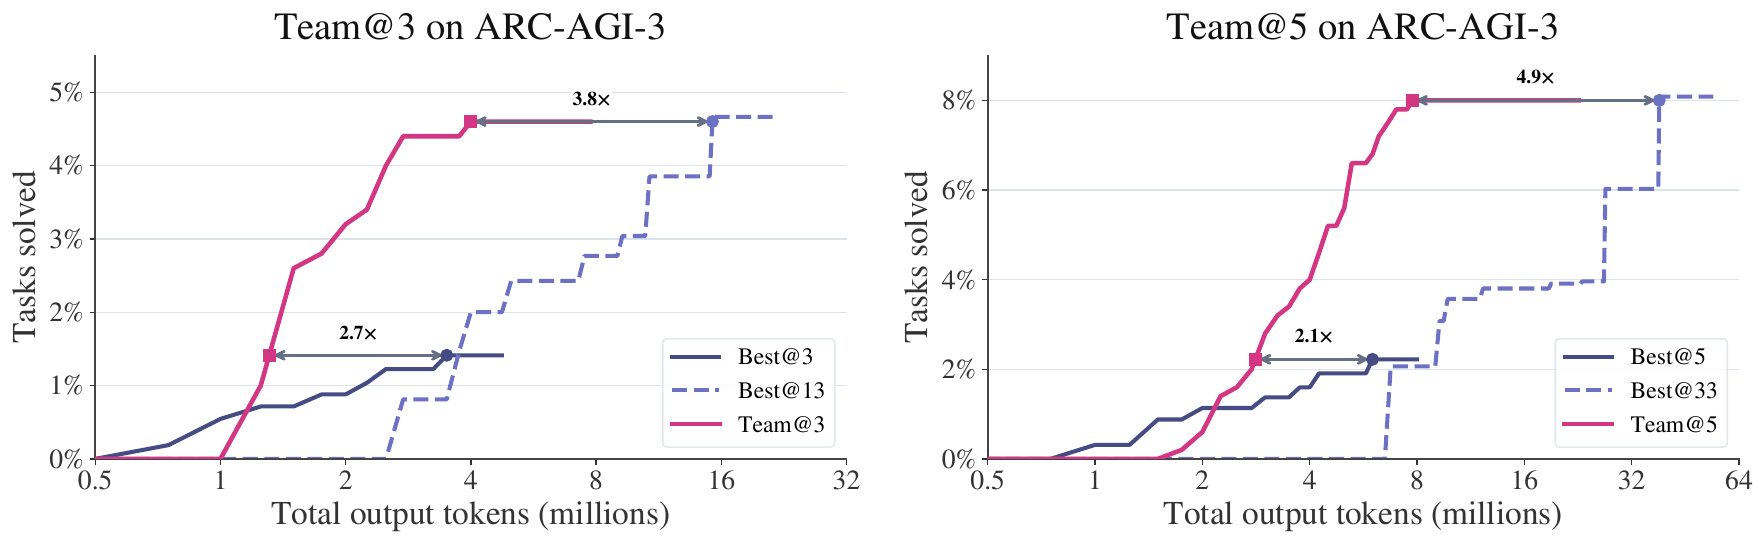
\includegraphics[width=.88\textwidth,height=.30\textheight,keepaspectratio]{figures/print/test-time-communication_fig3.png}
\caption{The value of communication can change with the budget. In the reported ARC-AGI-3 experiments, independent attempts lead at small total output-token budgets, while communicating teams reach higher success later. This within-study comparison retains the original task and resource axis; it is not a pooled scaling curve. Source: \citet{test-time-communication}, arXiv:2609.21032, Figure 3, CC BY 4.0. Blank margins trimmed; image content unchanged.}
\label{fig:atlas-communication}
\end{figure*}

\subsection{Learned coordination changes the comparison}
Kimi K2.5 trains a controller through reinforcement learning while helpers remain fixed. Its reward design addresses both a controller that refuses to delegate and one that creates unproductive parallel activity \citep{kimi-agent-swarm}. The reported BrowseComp gain depends strongly on the single-agent baseline: against a single agent with context cleaning, the advantage is 3.5 points (78.4\% versus 74.9\%), and the larger gap against 60.6\% without context management partly reflects context handling rather than delegation.

Two preprints from October and November train the coordination policy itself. In MPT (Harvard University), agents bid for the next turn, and post-training learns bids and actions together \citep{mpt-self-orchestration}. On 50 held-out deep-research questions, each averaged over three runs, accuracy is $21.0\pm4.1\%$ versus $9.0\pm2.1\%$ for monolithic reinforcement learning. With action policies held fixed, learned turn allocation reaches a mean reward of 41.5 against 25.4 for the strongest alternative coordination scheme over 32 crafting worlds. The three roles are supplied by the researchers; what is learned is when each acts. In s$^3$ (University of Washington and the Allen Institute for AI), agents with a shared team reward learn when to work alone and when to read others' messages \citep{s3-swarm-scaling}. On an information-aggregation task, swarms trained with four agents and evaluated with eight succeed more than twenty times as often as online supervised fine-tuning, the strongest baseline, at matched training and inference budgets. In an exploration task, communication nearly halves repeated work relative to agents that do not communicate. Avalon-M1 is a third case: every agent in its organizations receives the same collective advantage during training, so organizational behavior is optimized together with task skill \citep{avalon-m1}.

WideSeek-R1 and Orchestra-o1 also train components of an orchestrated workflow, while Conductor learns which model to use in a bounded sequence \citep{wideseek-r1,orchestra-o1,sakana-conductor}. A complete comparison separates the base model, the learned controller, the available workers, and the training data. If the multi-agent system uses stronger helpers or additional trajectory supervision, replacing the graph alone does not identify the source of its gain, and training cost lies outside most inference-budget comparisons.

\subsection{Scaling laws and large demonstrations}
Ord fits an effective parallelization exponent to OpenAI's published GPT-5.6 Sol curves: at a fixed token budget per agent, a swarm of $N$ agents performs like one agent thinking $N^{\lambda}$ times longer \citep{ord-swarm-scaling}. Regressions on the published charts give $\lambda=0.68$ for BrowseComp, $0.57$ for SEC-Bench Pro, and $0.48$ for Terminal-Bench. At $\lambda=0.57$, sixteen agents equal one agent thinking about 4.9 times longer. The exponents are estimates from interpolated curves for one model family, one hierarchical design, and few group sizes; no new runs at matched total budgets were made. Extrapolating them to thousands of agents would require task dependency structure and coordination efficiency to stay stable over orders of magnitude.

Economic analyses of parallel research make this assumption consequential: growth depends on how the technology for dividing and integrating work changes, not only on the number of researchers \citep{trammell-parallelizability}. Theoretical superlinear scenarios and forecasts remain hypotheses \citep{bradshaw-swarm-exponent} to be compared with measured frontiers.

Large campaigns establish feasibility under their reported conditions. OpenAI's Navier--Stokes campaign reports a successful group on the order of 10,000 concurrent agents, substantial messaging and token use, and a formalized mathematical result, without a matched single-agent or smaller-team run \citep{openai-navier-stokes}. Anthropic's 1,000-agent Fable 5.2 team reproduced the formal proof of Fermat's Last Theorem in 28.7 hours \citep{anthropic-fable-team-scaling}. The September formalization it is compared with was written in 11 days by a researcher and dozens of agents on a model roughly comparable to Fable 5.1, using the Prove2Me platform and about 6 billion output tokens \citep{fermat-last-theorem}; the November run used one-third as many output tokens and wrote a proof one-seventh as long. The comparison is not independent of the earlier work: the November team received 60 target statements, a one-sentence sketch of the classical route, the definitions the statements use, and 47 lemmas already proved in the September formalization. Model version, harness, and human direction also changed, and the authors call the run a toy experiment. SwarmEvolve (Brown University) runs hundreds of low-cost agents per round that exchange KV caches instead of text; on 21 problems in mathematical discovery and scientific computing it needs a median of 4 to 8 minutes with Qwen3-8B, and 3 to 6 minutes with larger models, to reach the best scores that text-based evolutionary frameworks reach in 60 minutes \citep{swarmevolve}. The zeta-function and cryptographic campaigns likewise combine strong models, human choices, long inference, and many workers \citep{riemann-zeta-swarm,crypto-weaknesses}. Such demonstrations motivate controlled scaling studies; they do not supply the missing counterfactual.
